\documentclass[11pt]{article}
\usepackage{amsmath,textcomp,amssymb,geometry,graphicx,tikz,cancel,color}
\usepackage{algpseudocode,algorithm}
\usepackage[T1]{fontenc}
\usepackage[colorlinks=true,urlcolor=blue]{hyperref}

\def\Name{Zackery Field}  % Your name
\def\Sec{}  % Your GSI's name and discussion section
\def\Login{} % Your login
\def\Homework{5}%Number of Homework
\def\Session{Spring 2014}

\title{Lab 5: Protein Structure Prediction}
\author{\Name}%, section \Sec, \texttt{\Login}}
\markboth{--\Session\  Homework \Homework\ \Name, section \Sec}
{\Session\ Homework \Homework\ \Name, section \Sec, \texttt{\Login}}
%\pagestyle{myheadings}

\begin{document}
\maketitle

\section*{Part 0\footnote{Nice use of zero-indexing.}:   Examine \href{http://www.uniprot.org/uniprot/P71707}{sequence record} for PBP1A\_MYCTU}

The header of the sequence file reveals that the record is in the manually curated SwissProt
section:  "P71707 (PBP1A\_MYCTU) Reviewed, UniProtKB/{\bf Swiss-Prot}".

\subsection{TMHMM comparison}

TMHMM and Uniprot both predict a helical TM region at residues 139-159.\footnote{It is possible that the results from TMHMM/Pfam and Uniprot are related, because
the Uniprot record could have been populated with data from both Pfam and TMHMM.}

\href{http://www.uniprot.org/uniprot/P71707}{UniProt}: Transmembrane - Helical 139-159

\href{http://www.cbs.dtu.dk/cgi-bin/webface2.fcgi?jobid=5318B8E100002CA9C6B99942&wait=20}{TMHMM}:   Transmembrane - Helical 137-159

\subsection{Pfam comparison}

The Pfam-A matches discovered using the \href{http://pfam.sanger.ac.uk/search/sequence}{Sequence Search} tool
shows that their is agreement between the Pfam and Uniprot records. Both records 
place a \href{http://pfam.sanger.ac.uk/family/PF00912.17}{transglycosylase} at 
region 180-360 (aa). Both records also show a \href{http://pfam.sanger.ac.uk/family/PF00905.17}{transpeptidease}
at region 453-734 (aa).


\section*{Part 1: \href{http://www.sbg.bio.ic.ac.uk/phyre2/phyre2_output/083b01625d2f5d9b/summary.html}{Phyre-results}}

\section*{Part 2: Run BLAST vs PDB at NCBI}

\begin{figure}[h!]
\centering
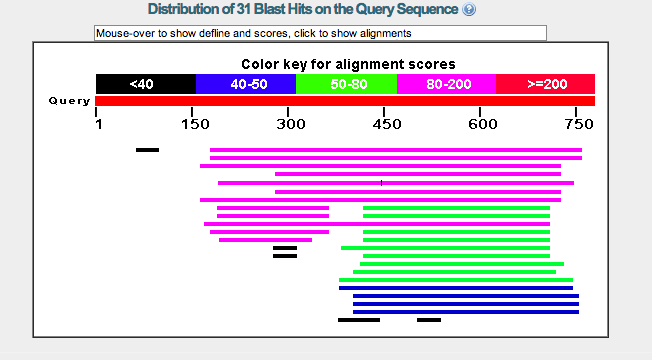
\includegraphics[scale=0.75]{Blast-vs-pdb-p71707.png}
\caption{A screenshot of the alignment overlap display from a blast query of 
p71707 run against the pdb database.}
\end{figure}

Top Hit: \href{http://www.ncbi.nlm.nih.gov/protein/208435656?report=genbank&log$=prottop&blast_rank=1&RID=HHF3ZR95015$}{3DWK\_A}

The Pfam analysis of both the top hit and the target are in agreement. Both
Pfam analyses describe approximately the same MDA. That is to say both a 
\href{http://pfam.sanger.ac.uk/family/PF00912.17}{transglycosylase} and a 
\href{http://pfam.sanger.ac.uk/family/PF00905.17}{transpeptidease}
are identified, but 3DWK\_A does not have an N terminal region extending from the
transglycosylase, whereas p71707 does. 

The transglycosylase region of p71707 is from residues 180-360.
The transglycosylase region of 3DWK\_A is from residues 15-191.

The BLAST pairwise alignment for those regions:

\begin{verbatim}
Query  182  EIAKIVPPEGNRVDVNLSQVPMHVRQAVIAAEDRNFYSNPGFSFTGFARAVKNNLFGG-D  240
            E+ K +        VNL  VP  ++ AV+A ED  FY +    +     A+  NL GG  
Sbjct  16   ELVKTLDNGQRHEHVNLKDVPKSMKDAVLATEDNRFYEHGALDYKRLFGAIGKNLTGGFG  75

Query  241  LQGGSTITQQYVKNALVGSAQHGWSGLMRKAKELVIATKMSGEWSKDDVLQAYLNIIYFG  300
             +G ST+TQQ VK+A +  +QH   G  RKA+E  ++ ++  E+SKDD+ Q YLN IY+ 
Sbjct  76   SEGASTLTQQVVKDAFL--SQHKSIG--RKAQEAYLSYRLEQEYSKDDIFQVYLNKIYYS  131

Query  301  RGAYGISAASKAYFDKPVEQLTVAEGALLAALIRRPSTLDPAVDPEGAHARWNWVLDGMV  360
             G  GI AA+K YF+K ++ L +AE A LA L + P+  +    P+ A  R N VL  M 
Sbjct  132  DGVTGIKAAAKYYFNKDLKDLNLAEEAYLAGLPQVPNNYNIYDHPKAAEDRKNTVLYLMH  191
\end{verbatim}

A BLAST alignment was done on these two regions in particular and 
the results were: Max Score 93.6 Total Score: 93.6 Query cover: 97\% E-value: 1e-28 Ident: 33\%.

Since the sequence identity is on the upper edge of the twilight zone of protein sequence
alignments (20-35\%PID) 
\footnote{\href{http://peds.oxfordjournals.org/content/12/2/85.full}{Twilight zone of protein sequence alignments}}, 
with high sequence coverage it is possible that these two regions do not represent the same transglycosylase domain. 
However, as the twilight paper states, more than 95\% of sequences above 30\% PID
were homologus. Therefore, I would agree with the Pfam classification that both of 
these regions contain a domain from the transglycosylase family. 

The transpeptidease region of p71707 is from residues 453-743.
The transpeptidease region of 3DWK\_A is from residues 294-562.

The BLAST pairwise alignment for those regions:

\begin{verbatim}
Query 453   VVSIDPHNGAVRAYYG  469
               +D   G + A  G
Sbjct 294   ATILDSKTGGLVAISG  310

Query  470  G-DNANGFDFAQAG--LQTGSSFKVFA----LVAALEQGIGLGYQVDSSPLTVDGIKITN  522
            G D  +  +  QA     TGSS K F      +  ++       Q D S   VDG    N
Sbjct  311  GRDFKDVVNRNQATDPHPTGSSLKPFLAYGPAIENMKWATNHAIQ-DESSYQVDGSTFRN  369

Query  523  VEGEGCGTCNIAEALKMSLNTSYYRLM--LKLNGGPQAVADAAHQAGIASSFPGVAHTLS  580
             + +  GT +I +AL+ S N    +    +K N G  A    A + G           L+
Sbjct  370  YDTKSHGTVSIYDALRQSFNIPALKAWQSVKQNAGNDAPKKFAAKLG-----------LN  418

Query  581  EDGKGGPPNNGIVLGQYQTRV--IDMASAYATLAASGIYHPPHFVQKVVSANGQVLFDAS  638
             +G  GP     VLG   +      +ASA+A +A  G Y+  H +QKVV+ +G+ +    
Sbjct  419  YEGDIGPSE---VLGGSASEFSPTQLASAFAAIANGGTYNNAHSIQKVVTRDGETIEYDH  475

Query  639  TADNTGDQRIPKAVADNVTAAMEPIAGYSRGHNLAGGRDSAAKTGTTQFGDTT-------  691
            T+           +A+ +    +P  G + GH ++ G +  AKTGT  +G  T       
Sbjct  476  TSHKAMSDYTAYMLAEMLKGTFKPY-GSAYGHGVS-GVNMGAKTGTGTYGAETYSQYNLP  533

Query  692  --ANKDAWMVGYTPSLSTAVWVGTVK----GDEPLVTASGAAIYGSGLPSDIWKATMDGA  745
              A KD W+ G+TP  + +VW+G  K    G+   V  S         P  +++  M   
Sbjct  534  DNAAKDVWINGFTPQYTMSVWMGFSKVKQYGENSFVGHSQQE-----YPQFLYENVM-SK  587
\end{verbatim}

A BLAST alignment was done on these two regions in particular and the results 
were: Max Score 69.3 Total Score: 69.3 Query cover: 79\% E-value: 3e-18 Ident: 29\%.

Since the sequence identity is well within the twilight zone of protein sequence
alignments (20-35\%PID) 
it is possible that these two regions do not represent the same transpeptidease domain. 
Since this 29\% identity is only over 80\% of the sequence, the PID is actually lower.
As the twilight paper states, more than 90\% of sequences below 25\% PID
were not homologus. I would not agree with the Pfam classification that both of 
these regions contain a transpeptidease domain. The E-value for the transpeptidease 
prediction for p71707 (9.1e-50) is 18 orders of magnitude lower than the E-value for the transpeptidease
prediction for 3DWK\_A (1.5e-32). Therefore, the transpeptidease classification for
p71707 should remain, and the transpeptidease classification for 3DWK\_A is more 
likely to be incorrect.


\begin{figure}[h!]
\centering
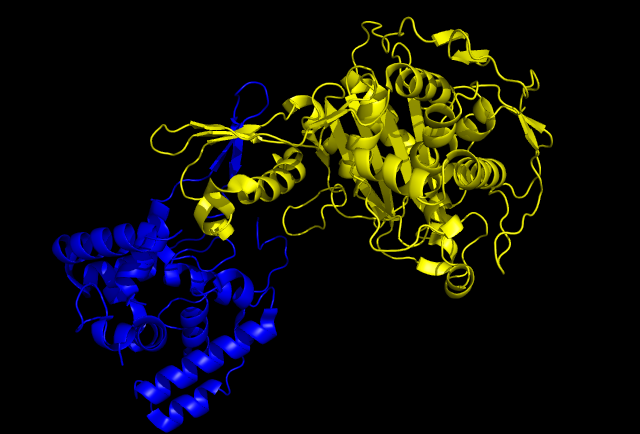
\includegraphics[scale=0.5]{3dwk_domains.png}
\caption{An image of the 3d structure of 3DWK\_A with the Pfam identified domains
highlighted. {\color{blue}{Blue}}: \href{http://pfam.sanger.ac.uk/family/PF00912.17}{transglycosylase}; 
{\color{yellow}{Yellow}}:\href{http://pfam.sanger.ac.uk/family/PF00905.17}{transpeptidease}}
\end{figure}

\section*{Part 3: Homolog selection, MSA Construction }

\subsection{Run Uniprot BLAST. Pull all sequences identified}

\subsection{Construct MSA with MAFFT}

\subsection{}
\end{document}
Query for transpeptidease domain: VVSIDPHNGAVRAYYGGDNANGFDFAQAGLQTGSSFKVFALVAALEQGIGLGYQVDSSPLTVDGIKITNVEGEGCGTCNIAEALKMSLNTSYYRLMLKLNGGPQAVADAAHQAGIASSFPGVAHTLSEDGKGGPPNNGIVLGQYQTRVIDMASAYATLAASGIYHPPHFVQKVVSANGQVLFDASTADNTGDQRIPKAVADNVTAAMEPIAGYSRGHNLAGGRDSAAKTGTTQFGDTTANKDAWMVGYTPSLSTAVWVGTVKGDEPLVTASGAAIYGSGLPSDIWKATMDGA

Target for transpeptidease domain: ATILDSKTGGLVAISGGRDFKDVVNRNQATDPHPTGSSLKPFLAYGPAIENMKWATNHAIQDESSYQVDGSTFRNYDTKSHGTVSIYDALRQSFNIPALKAWQSVKQNAGNDAPKKFAAKLGLNYEGDIGPSEVLGGSASEFSPTQLASAFAAIANGGTYNNAHSIQKVVTRDGETIEYDHTSHKAMSDYTAYMLAEMLKGTFKPYGSAYGHGVSGVNMGAKTGTGTYGAETYSQYNLPDNAAKDVWINGFTPQYTMSVWMGFSKVKQYGENSFVGHSQQEYPQFLYENVMSK
